% This is samplepaper.tex, a sample chapter demonstrating the
% LLNCS macro package for Springer Computer Science proceedings;
% Version 2.20 of 2017/10/04
%
\documentclass[runningheads]{llncs}
%
% A lot of package loading
\usepackage[pdftex]{graphicx}
\usepackage{geometry}
\usepackage[cmex10]{amsmath}
\usepackage{array, algpseudocode}
\usepackage{amsmath, amssymb, amsfonts, parskip, graphicx, verbatim}
\usepackage{url, hyperref}
\usepackage{bm, rotating, adjustbox, latexsym}
\usepackage{tabularx, booktabs}
\newcolumntype{Y}{>{\centering\arraybackslash}X}
\usepackage{float, setspace, mdframed}
\usepackage{color, contour, placeins, subfig, cite}
\usepackage[mathscr]{euscript}
\usepackage[osf]{mathpazo}
\usepackage{pgf, tikz, microtype, algorithm}
\usetikzlibrary{shapes,backgrounds,calc,arrows}
\usepackage{xcolor, colortbl, dsfont}


% If you use the hyperref package, please uncomment the following line
% to display URLs in blue roman font according to Springer's eBook style:
\renewcommand\UrlFont{\color{blue}\rmfamily}

\graphicspath{{figures/}}

\begin{document}
%
\title{Shark Smell Optimization}
%

%\titlerunning{Abbreviated paper title}
% If the paper title is too long for the running head, you can set
% an abbreviated paper title here
%
\author{Jochem Ram (S2040328), Jerry Schonenberg (S2041022), Wouter van Tol (S2041340), Thomas Wink (S1705148)}
%


\authorrunning{J. Ram, J. Schonenberg, et al.}
% First names are abbreviated in the running head.
% If there are more than two authors, 'et al.' is used.
%
\institute{Leiden Institute of Advanced Computer Science, The Netherlands}
%
\maketitle              % typeset the header of the contribution
%


\begin{abstract}
In this paper an optimization algorithm is presented which is based on the way sharks find their pray. This algorithm, which was first proposed in another paper\cite{abedinia2014shark}, gradient-based general searches and a set of local searches. We present the pseudocode along with a list of all used functions and deviations from the original paper. We show an ECDF and ERT plot in which we compare SSO with BIPOP\cite{COCOperformace} in 20 dimensions. We see that our algorithm performs worse than BIPOP on almost every function, and also performs worse than the algorithm in the original paper. This is because the original paper did not specify a lot of details causing us to struggle with the implementation. 
\end{abstract}





\section{Introduction}
For as long as humans exist, we have looked at nature for inspiration. Most inventions humans have made come from investigating natural phenomena and trying to reproduce what we see. This is still the case nowadays, where we think we know almost everything. It has proven useful to examine the way processes happen in nature and to try to implement this in problems we have ourselves. One example is to look at the way a shark, one of the best hunters in the sea, finds a pray in an efficient way. This can be used in an optimization problem to quickly find the best solution to a complex problem in a high dimensional solution space.\\
In this paper we present the findings of the shark-smell-optimization (SSO)\cite{abedinia2014shark} algorithm. This will be done using IOHprofiler by comparing the performance of the algorithm for different objective functions.

\section{Algorithm Description} \label{sec:description}
This algorithm uses a "shark", an individual, to find a "wounded fish", the maximal value of the objective function, by following the "blood particles", the gradient of the objective function, and performing "circular searches", local searches around the individual's position at each stage. This is repeated for each individual until stage $k_{max}$ is reached. The number of individuals and stages can be decided by the user. \\
A single iteration of the algorithm will first contain the calculation of the movement of the individuals in each dimension of the search space. Then a new position is calculated for every position. From this position a random local search will be done, where the best point from this search will be compared with the position from the the first search. The best one of these will be the new starting position for this individual for the next iteration.


\subsection{Comparison with standard algorithms}
The SSO algorithm can be best compared to simulated annealing. This algorithm is based on the concept of heat treatment in metals, in which a hot metal is slowly heated to let the atoms slowly settle to minimal energy states. This is used in optimization by perturbing each point randomly and choosing whether to move to that point or not. If the objective function in that point is higher, it will always move. If the objective function is lower, the chance of movement is calculated with the difference in the objective function values.\\
This algorithm matches the closest to SSO because, unlike almost all natural optimization algorithms, these two algorithms are not based on mutation or swarm behavior. They are based on the searches of individual candidate solutions without any communication between the individuals. Also, introduce randomness in their search pattern. SSO does this by choosing random values around the solution candidate and evaluating all of them at once and simulated annealing does this by choosing a random value around the solution candidate and evaluating immediately. For simulated annealing this leads to a higher chance of reaching a local minimum, but this is mitigated by offering the chance of a restart where an individual is placed back to a previously found significantly better solution candidate.\\
However, where the SSO uses the gradient to find the movement direction of the search point, simulated annealing uses difference in objective function values in two points. Also, SSO can not move to a position with a lower objective function value while for simulated annealing this is one of it's strengths.\\


\section{Pseudo-code}
\label{secPseu}
We followed the following notation convention. All user assigned variables are mentioned in Appendix A.
\subsection{Variable explanation}
\begin{itemize}
    \item $N$: The number of individuals in the set/array. This number should be higher or equal to 1.
    \item $M$: The dimensionality of the search space.
    \item $k_{max}$: Maximal amount of stages. This number should be at least one.
    \item $O$: Number of rotational candidate solutions.
    \item $n$, $m$, $k$ and $o$: Administrative array counters for $N$, $M$, $k_{max}$ and $O$ respectively.
    \item $X_n^k$: The solution candidate $\mathds{R}^M$ of an individual at a stage.
    \item $V_n^k$: The calculated movement in $\mathds{R}^M$ for an individual at a stage.
    \item $v_{n,m}^k$: The calculated movement in a direction for an individual at a stage.
    \item $Y_n^k$: The provisional solution candidate in $\mathds{R}^M$ after movement of an individual at a stage.
    \item $Z_n^{k}$: Set of O provisional solution candidates in $\mathds{R}^M$ of an individual at a stage after local search.
    \item $x_m$: A variable in the search space.
    \item $x_m^{\text{min}}$, $x_m^{\text{max}}$: The minimal and maximal values in the search space for a variable.
    \item $f(\mathbf{x})$: Objective function value of $\mathbf{x}$ ($f: \mathds{R}^M \rightarrow \mathds{R})$.
    \item $\leftarrow$: Assignment operator.
    \item $\boldsymbol{\alpha}$: User assigned vector in $\mathds{R}^{k_{max}}$. Represents the inertia coefficient for each stage. These numbers should be in the range [0, 1]. Together with $\boldsymbol{\eta}$ it should be 1.
    \item $\boldsymbol{\beta}$: User assigned vector in $\mathds{R}^{k_{max}}$. Represents the velocity limiter ratio for each stage. This number should be higher than 0.
    \item $\boldsymbol{\eta}$: User assigned vector in $\mathds{R}^{k_{max}}$. Limits the gradient of the objective function for each stage. These numbers should be in the range [0, 1]. Together with $\boldsymbol{\alpha}$ it should be 1.
    \item $ r1 $ and $r2 $: Random uniform value between $ 0 $ and $ 1$ to give the algorithm more stochastic search value.
    \item $ R3 $: Vector in $\mathds{R}^M$ with random uniform values between $ -1 $ and $ 1$ to give the algorithm more stochastic search value.
    \item $\arg \max() $: Takes the variable with the highest objective function value.
    \item $\arg \max_{a=1}^A()$: Iterates over a and takes the variable with the highest objective function value.
    \item Further notation convention is based on mathematics.
\end{itemize}

\subsection{Used functions}

1) $
v_{n,m}^k \leftarrow \eta _k \cdot r1 \cdot  \left. \frac{\partial f(x)}{\partial x_m} \right \rvert_{X_{n}^k} + \alpha_k \cdot r2 \cdot v_{n,m}^{k-1}
$ \\ \\
This function is the calculation of movement in dimension m for individual n in stage k. In the first term of the calculation we take the partial derivative of the objective function to $x_m$, and then multiply it with a velocity limiter constant and a random value for extra stochastic search value. In the second term we take the movement from the last stage in this dimension for this individual and multiply it with a random value and an inertia constant. This function is used in line \ref{eq:1}. \\ 

2) $
\left \lvert v_{n,m}^k \right \rvert  > \left \lvert \beta_k \cdot v_{n,m}^{k-1} \right \rvert
$ \\ \\
This line limits the acceleration of the movement of an individual in dimension m. This is done by comparing the new velocity to the velocity in the previous stage multiplied with a velocity limiter constant. This function is used in line \ref{eq:2}. \\ 

3) $
Y_n^{k+1} \leftarrow X_n^k + V_n^k
$ \\ \\
Assignment of provisional new location based on previous location and movement. This function is used in line \ref{eq:3}. \\ 

4) $
Z_n^{k+1, o} \leftarrow Y_n^{k+1} + R3 \cdot V_n^{k}
$ \\ \\
This function finds $O$ new solution candidates in a local search in the vicinity of $Y_n^{k+1}$. This is done with the provisional new position Y, and the velocity of this stage multiplied with a random vector R3. This function is used in line \ref{eq:4}.\\

5) $
X_n^{k+1} \leftarrow \arg \max (\arg \max_{o=1}^O(f(Z_n^{k+1, o})),f(Y_n^{k+1}))
$ \\ \\
This function finds the best new location by comparing the provisional new location with the solution candidates from the local search, and testing their objective function value. This function is used in line \ref{eq:5}.



\newpage
\subsection{Pseudocode}
\vspace{-4mm} 
\begin{algorithm}[!h]
\begin{algorithmic}[1]
    \State{$N \leftarrow User \quad assigned$} \Comment{Initialize} 
    \State{$ k_{max} \leftarrow User \quad assigned $}
    \State{$ k \leftarrow 1$ }
    \State{$ O \leftarrow User \quad assigned $ }
    \State{$ \boldsymbol{\alpha} \leftarrow User \quad assigned $}
    \State{$ \boldsymbol\beta \leftarrow User \quad assigned $}
    \State{$ \boldsymbol\eta \leftarrow User \quad assigned $}
	\For{$n = 1 \rightarrow n $}
	    \For{$m = 1\rightarrow m$}
	        \State{$x_{n,m}^1 \leftarrow \bm{\mathcal{U}}(x_m^{\text{min}},x_m^{\text{max}})$}
	    \EndFor
	\EndFor
	\While{$k\leq k_{max}$}
    	\For{$n = 1 \rightarrow N$}  \Comment{Calculation of movement per individual} 
    	    \For{$m = 1\rightarrow M$}
    	        \State{$v_{n,m}^k \leftarrow \eta _k \cdot r1 \cdot  \left. \frac{\partial f(x)}{\partial x_m} \right \rvert_{X_{n}^k} + \alpha_k \cdot r2 \cdot v_{n,m}^{k-1}$}\label{eq:1}
    	        \If{$\left \lvert v_{n,m}^k \right \rvert  > \left \lvert \beta_k \cdot v_{n,m}^{k-1} \right \rvert $}\label{eq:2}
    	            \State{$ v_{n,m}^k \leftarrow  \beta_k \cdot v_{n,m}^{k-1}  $}
    	       \EndIf
    	    \EndFor
    	\EndFor
    	\For{$n = 1 \rightarrow N$}  \Comment{Provisional assignment of new position per individual} 
    	    \State{$Y_n^{k+1} \leftarrow X_n^k + V_n^k$}\label{eq:3}
    	\EndFor
    	\For{$n = 1 \rightarrow N$} \Comment{Random local search from provisional position per individual} 
    	    \For{$o = 1 \rightarrow O$}
    	        \State{$Z_n^{k+1, o} \leftarrow Y_n^{k+1} + R3 \cdot V_n^{k}$} \Comment{Deviation \label{dev}}\label{eq:4}
    	    \EndFor
    	\EndFor
    	\For{$n = 1 \rightarrow N$} \Comment{Definitive assignment of new position per individual} 
    	   % \For{$o = 1 \rightarrow O$}
    	        \State{$X_n^{k+1} \leftarrow $ $\max (\max_{o=1}^O(f(Z_n^{k+1, o})),f(Y_n^{k+1}))$}\label{eq:5}
    	   % \EndFor
    	   % \State{$X_n^{k+1} \leftarrow $ max($f(X_n^{k+1}), f(Y_n^{k+1})$)}
    	\EndFor
    	\State{$k \leftarrow k+1$} \Comment{Administration}
    \EndWhile
 \end{algorithmic}
\caption{Shark Smell Optimization}
\label{Alg:SSO}
\end{algorithm}
\vspace{-2mm}


\newpage
\section{Assumptions}
For this algorithm we assumed that the objective function should be maximized.\\
In our pseudocode, on line \ref{dev}, we deviated from the original paper. In the original paper this line was: \\
$Z_n^{k+1, o} \leftarrow Y_n^{k+1} + R3 \cdot Y_n^{k+1}$ \\\label{assumption}
We changed the second $ Y $ to a $V$:\\
$Z_n^{k+1, o} \leftarrow Y_n^{k+1} + R3 \cdot V_n^{k+1}$ \\
We did this as we think that the searchspace for the rotational movement should be related to the velocity, and not to the current location. Otherwise we would be placing the random local search points on a line through the origin, which is arbitrary. \\
On this line we also changed $R3$ to be a vector instead of a number, since this means the rotational search is not just in the direction of the movement but also in other directions. \\
Since the velocity is based on the previous velocity, and can maximally be 4 times as large, we need an initial velocity unequal to 0 or else every new velocity will also be 0. The paper has not mentioned which value they used. We think that it should be a small number compared to the searchspace, so we chose $V_{n,m}^0 = (x_m^{max} - x_m^{min})/100$.\\
Furthermore, many details were not explained in the original paper such as the chosen values for $N$, $k_{max}$, $O$, or the implementation of the partial derivative. We empirically chose the highest numbers for the constants for which the algorithm still computed quickly enough.\\

\subsection{Problems with implementation derivative}
In the paper, the velocity is linearly equated to the derivative. This is a problem since his would mean that for a function with range 10 and function values in the millions, such as the second function with which we test the algorithm, the derivative will be in the millions and thus the velocity as well. We should, however, be changing our position with a value between 0 and 5. The other way around, if the range is in the millions and the function ranges between 1.0 and 2.0, the derivative is too low for the individual to reach the optimum within limited stages.\\
Also, for a first order approximation of a partial derivative we take the value at a point and the value at that point plut a small distance $d$. How small this distance is, is very important for the speed and accuracy of the algorithm but was not explained by the paper. This value should also gradually become lower as the individual approaches the optimum, such that the evaluation point does not overshoot the optimum.\\


\section{Experiments}
To test the algorithm we use IOHexperimenter for benchmarking and IOHanalyzer to process the data. These are both contained in the tool IOHprofiler\cite{IOHprofiler}.\\
The benchmarking with IOHexperimenter is done across 24 functions with each 5 instances and 3 runs per instance. The tests are done in 5 dimensions and 20 dimensions. The constants we used are shown in table \ref{tab:constants}.
\begin{table}[h!]
    \centering
    \begin{tabular}{c|c}
        Constant & Value \\ \hline \hline
        $N$ & 50\\\hline
        $k_{max}$ & 100\\\hline
        $O$ & 12 \\\hline
        $\alpha$ & 0.1 \\\hline
        $\beta$ & 4 \\\hline
        $\eta$ & 0.9
        \end{tabular}
    \caption{User assigned constants used in the algorithm}
    \label{tab:constants}
\end{table}{}

As for the implementation of the derivative, we did not scale the calculated velocity as to compensate for possible extreme values for the derivative. Instead we clamped the position of each individual within the searchspace and the overshoot of the derivative would very slowly be negated by the inertia term in line \ref{eq:1} of the pseudocode. Since this is not an optimal stagegy\\
We have tested the algorithm for both $d = (x_m^{max}-x_m^{min})/1000$ and $d = (x_m^{max}-x_m^{min})/1000000$.\\

To see how well the algorithm performed, we will compare it to BIPOP-CMA-ES\cite{COCOperformace} and create an Emperical Cumulative Distribution Function(ECDF)-plot for both these algorithms across all functions using the IOHanalyzer. This plot will show the performance of the algorithm compared to other algorithms in one glance.\\
To see the specific points at which the algorithm performs good or bad we will also make an Estimated Run Time-plot for each function.\\


\subsection{Original experiments}
The writers of the original paper did five experiments. In three of these experiments they compared SSO against the 32 most used algorithms in engineering applications. In these comparisons, the algorithm was the best, or equal to the best, in nearly every case. Only on one point did another algorithm perform better. Moreover, SSO was the fastest in each of these experiments. \\
In the other two experiments they compared SSO to three of the best performing algorithms. They did this by testing SSO on a testbed in 10- and 30-dimensional environments with 28 test functions. 5 of these functions are unimodal functions, 15 are multimodal functions and 8 are composition functions. In these two experiments, SSO performed significantly better.\\
In a final experiment they performed, they put SSO to the test on the real-world problem of PID-controller optimization. Here it outperformed all algorithms on two of the main objective functions in this field. SSO also had the least over- and undershoot in finding the PID-controller target value.

\section{Results}
After generating the data with the IOHexperimenter it was analysed by the IOHanalyzer.

\begin{figure}[h!]
    \centering
    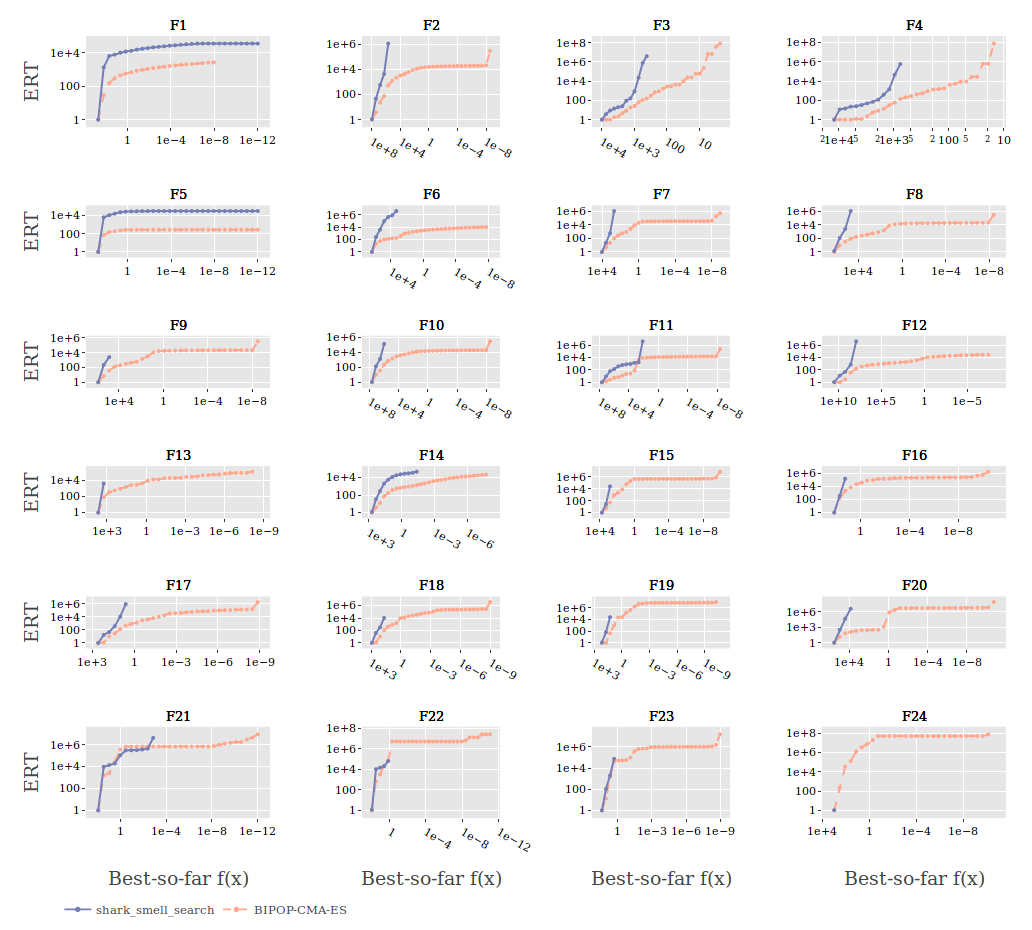
\includegraphics[scale =0.6]{D20-ERT.png}
    \caption{Estimated Run Time for 20 dimensions}
    \label{fig:ERT}
\end{figure}

\begin{figure}[h]
    \centering
    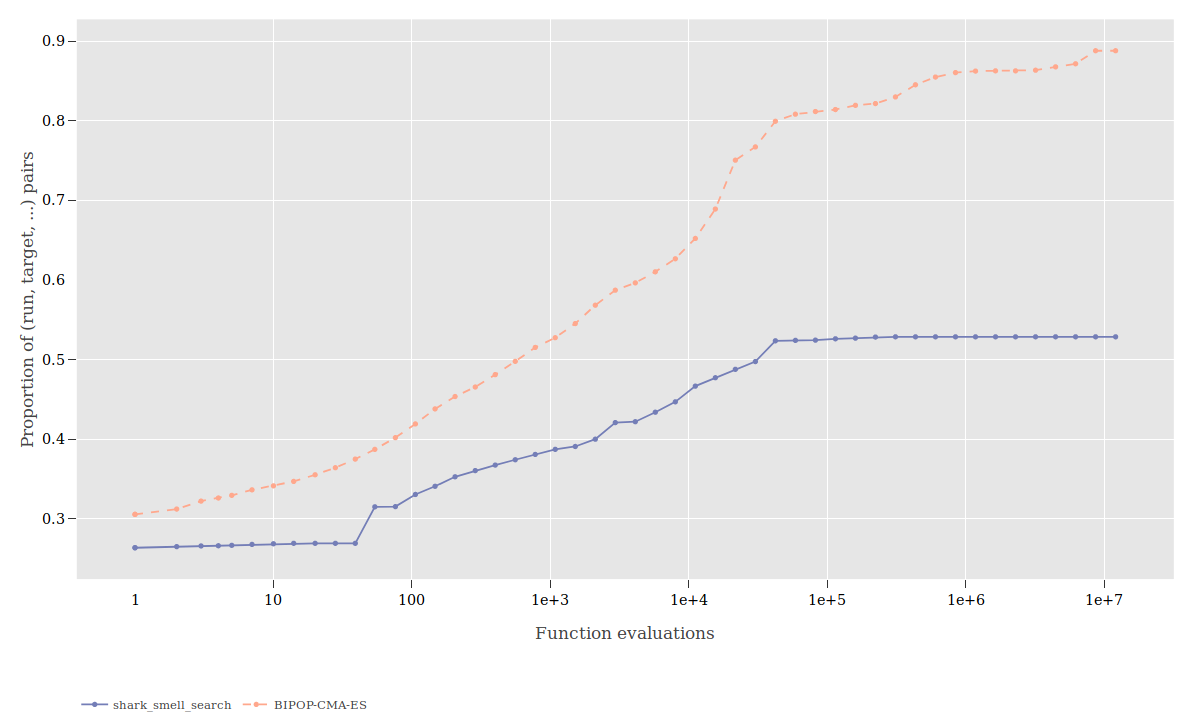
\includegraphics[scale = 0.4]{D20-ECDF.png}
    \caption{Empirical Cumulative Distribution Function for 20 dimensions}
    \label{fig:ECDF}
\end{figure}

In figure \ref{fig:ERT} we see the performance of the SSO in blue and the BIPOP algorithm in yellow. On the x-axes the deviation from the best objective function value reached is shown, and the y-axes show the estimated runtime needed to reach this value. This means that the lower the line stays, the quicker the algorithm reaches an optimum. Also, the farther right the line reaches, the closer the algorithm comes to the optimum.\\
It is clear that the SSO algorithm performs worse than the BIPOP algorithm on almost every function. However, SSO does quite well on f1, where it finds a better optimum, and f21, where it finds the local area of the optimum quicker. In f24 SSO does not even find a value other than the initialisation value, which is why SSO only has 1 point in this graph.\\
\\
To see how well the algorithm performs in general, we look at the ECDF-plot in figure \ref{fig:ECDF}. In this figure the x-axis shows the amount of evaluations and y-axis shows what proportion of the runs reached the target value for this amount of evaluations.
Therefore a steeper slope of the curve means that the algorithm performs better. Since the SSO line is below the BIPOP line on every point, SSO performs worse than BIPOP in general.\\
Both figures are shown for 20 dimensions, since the figures created for 5 dimensions are very similar and do not add information. \\


\section{Conclusion}
The original paper showed that the SSO algorithm performed better than all other algorithms it was compared to and for all functions that were tested. Since our algorithm performs much worse than BIPOP, even though the original paper did not compare SSO with BIPOP, we most likely implemented the algorithm in a different way which performs worse. The most obvious fault is the fact that we need to clamp the positions in the range to make sure the algorithm does not walk out of the searchspace. This most likely means that either the implementation of the algorithm has a fault or the scaling of the derivative to the velocity is implemented wrong. \\
Another explanation for the difference in performance between the original paper and our implementation is that the original paper has better results than they should have. This could be because of the assumption we made for the calculation of the provisional position\ref{assumption}. If the original paper did not make a typo but did in fact implement this and the function with which they tested their algorithm had their optimum in the origin, each rotational movement would find points between the individuals position and the origin, and therefore get closer to the origin for every rotational run. Since the origin is arbitrary, this would mean that the objective functions are chosen poorly and the algorithm accidentally finds the optimum because of this error.\\
We found that most parts of the algorithm were quite easy to implement, but it was difficult to implement the partial derivative and we quickly got a bit confused by the 3 and 4 dimensional arrays. We also found that it was difficult to find the right variables to use as there were some inconsistencies in the original paper with variable names. The algorithm itself is quite original as it is one of the only algorithms that we know of that does not use mutation or uses swarm mechanics. However, we do not think it is revolutionary because the concept is quite simple and it does not really negate problems with local minimums. 

\bibliographystyle{splncs04}
\bibliography{bibliography.bib}
\end{document}
